% !TeX program = xelatex
\documentclass[UTF8,a4paper,zihao=-4,fontset=none]{ctexart}
\setCJKmainfont[BoldFont={LXGW Neo XiHei}]{LXGW Neo ZhiSong}
\setCJKsansfont[AutoFakeBold=2]{LXGW Neo XiHei}
\setCJKmonofont{LXGW Neo XiHei}
\setCJKfamilyfont{zhhei}[AutoFakeBold=2]{LXGW Neo XiHei}
\providecommand{\heiti}{\CJKfamily{zhhei}}
% Shared renderer entrypoint for generated lessonplan.tex files.
% Generated documents should load ctexart, then input this file.

\usepackage{hepingjie_lessonplan}
% Hepingjie lesson-plan overlay coordinates.
% Coordinate origin: top-left corner of an A4 portrait page.
% Units: mm. These coordinates are frozen for templates/lessonplan/hepingjie_blank.pdf.

\newcommand{\LPBackgroundPdf}{templates/lessonplan/hepingjie_blank.pdf}

% Page 1 fixed fields.
\newcommand{\LPDateYearX}{65mm}
\newcommand{\LPDateMonthX}{89mm}
\newcommand{\LPDateDayX}{110mm}
\newcommand{\LPDateY}{38mm}
\newcommand{\LPRecordPageX}{170mm}
\newcommand{\LPRecordPageY}{38mm}

\newcommand{\LPTopicX}{32mm}
\newcommand{\LPTopicY}{49mm}
\newcommand{\LPTopicW}{108mm}
\newcommand{\LPTypeX}{154mm}
\newcommand{\LPTypeY}{49mm}
\newcommand{\LPTypeW}{40mm}

\newcommand{\LPUnitTotalX}{67mm}
\newcommand{\LPUnitTotalY}{61mm}
\newcommand{\LPTopicTotalX}{111mm}
\newcommand{\LPTopicTotalY}{61mm}
\newcommand{\LPCurrentPeriodX}{169mm}
\newcommand{\LPCurrentPeriodY}{61mm}

\newcommand{\LPBodyX}{33mm}
\newcommand{\LPObjectiveY}{74mm}
\newcommand{\LPObjectiveH}{39mm}
\newcommand{\LPKeyPointY}{119mm}
\newcommand{\LPKeyPointH}{15mm}
\newcommand{\LPDifficultyY}{137mm}
\newcommand{\LPDifficultyH}{15mm}
\newcommand{\LPMethodY}{156mm}
\newcommand{\LPMethodH}{15mm}
\newcommand{\LPMediaY}{174mm}
\newcommand{\LPMediaH}{15mm}
\newcommand{\LPBlackboardY}{196mm}
\newcommand{\LPBlackboardH}{73mm}
\newcommand{\LPBodyW}{164mm}

% Teaching process boxes on pages 2-4.
\newcommand{\LPProcessX}{33mm}
\newcommand{\LPProcessY}{31mm}
\newcommand{\LPProcessW}{163mm}
\newcommand{\LPProcessFullH}{249mm}
\newcommand{\LPProcessPageFourH}{160mm}


\usetikzlibrary{calc}
\begin{document}

\LPBackgroundPage{1}{
  \LPCenterBox{\LPDateYearX}{\LPDateY}{12mm}{5mm}{}
  \LPCenterBox{\LPDateMonthX}{\LPDateY}{10mm}{5mm}{}
  \LPCenterBox{\LPDateDayX}{\LPDateY}{10mm}{5mm}{}
  \LPCenterBox{\LPRecordPageX}{\LPRecordPageY}{10mm}{5mm}{1}
  \LPHeaderCell{\LPTopicX}{\LPTopicY}{\LPTopicW}{8mm}{有理数的大小比较}
  \LPHeaderCell{\LPTypeX}{\LPTypeY}{\LPTypeW}{8mm}{概念形成课}
  \LPCenterBox{\LPUnitTotalX}{\LPUnitTotalY}{12mm}{5mm}{7}
  \LPCenterBox{\LPTopicTotalX}{\LPTopicTotalY}{12mm}{5mm}{4}
  \LPCenterBox{\LPCurrentPeriodX}{\LPCurrentPeriodY}{12mm}{5mm}{4}
  \LPTextBox{\LPBodyX}{\LPObjectiveY}{\LPBodyW}{\LPObjectiveH}{\LPPlainLine{说出并解释数轴上的大小顺序，使用本节规范术语表达。}\LPPlainLine{按规范步骤完成利用数轴比较有理数大小，并说明关键依据。}\LPPlainLine{判断并订正与“负数大小比较中的绝对值反向关系”有关的常见错误。}\LPPlainLine{在变式或实际情境中运用本节方法，完整写出过程和结论。}}
  \LPTextBox{\LPBodyX}{\LPKeyPointY}{\LPBodyW}{\LPKeyPointH}{利用数轴比较有理数大小；两个负数绝对值大的反而小}
  \LPTextBox{\LPBodyX}{\LPDifficultyY}{\LPBodyW}{\LPDifficultyH}{负数大小比较中的绝对值反向关系}
  \LPTextBox{\LPBodyX}{\LPMethodY}{\LPBodyW}{\LPMethodH}{问题引导；比较归纳；正反例辨析}
  \LPTextBox{\LPBodyX}{\LPMediaY}{\LPBodyW}{\LPMediaH}{PPT；黑板；反馈卡；步骤卡}
  \LPTextBox{\LPBodyX}{\LPBlackboardY}{\LPBodyW}{\LPBlackboardH}{\LPBoardTitle{有理数的大小比较}\LPBoardLine{1}{核心：数轴上右边的数大；正数大于 $0$，$0$ 大于负数；两个负数绝对值大的反而小。}\LPBoardLine{2}{方法：统一表示形式后，优先用数轴位置或负数绝对值规则比较。}\LPBoardLine{3}{例题：比较 $-3$ 与 $-7$。 答：$|-3|=3<7=|-7|$，所以 $-3>-7$。}\LPBoardLine{4}{易错：错解：因为 $8>3$，所以 $-8>-3$。 纠正：错误；两个负数绝对值大的反而小，应为 $-8<-3$。}\LPBoardLine{5}{检查：条件、依据、步骤、符号或单位逐项核对。}}
}

\LPBackgroundPage{2}{
  \LPProcessBox{\LPProcessX}{\LPProcessY}{\LPProcessW}{\LPProcessFullH}{\LPProcessRow{情境引入}{\LPTeacherPart{问题}{清晨气温 $-5^\circ\mathrm C$，中午为 $2^\circ\mathrm C$，哪个温度高？怎样从数轴说明？}\LPTeacherPart{组织}{出示题目或情境，先让学生独立判断，再请两名学生说明依据。}\LPTeacherPart{说明}{数轴上 $2$ 在 $-5$ 右侧，所以 $2>-5$。}\LPTeacherPart{纠错}{若学生只报结论，追问基准、条件或运算依据，要求补成完整句。}\LPTeacherPart{归纳}{把情境中的信息转化为数学对象和关系。}\LPTeacherPart{意图}{用具体问题激活先修经验，并明确本节需要解决的核心矛盾。}}{\LPStudentPart{活动}{独立观察或计算，圈出关键信息后口头说明。}\LPStudentPart{预期}{数轴上 $2$ 在 $-5$ 右侧，所以 $2>-5$。}}{5}
\LPProcessRow{比较与抽象}{\LPTeacherPart{问题}{有理数大小比较有哪些规则？}\LPTeacherPart{组织}{组织观察、比较或试算，板书学生给出的共同点，并逐项核对术语。}\LPTeacherPart{说明}{数轴上右边的数大；正数大于 $0$，$0$ 大于负数；两个负数绝对值大的反而小。}\LPFigureBlock{
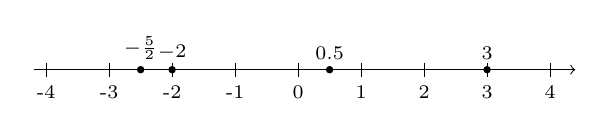
\begin{tikzpicture}[x=8mm,y=8mm,baseline=(current bounding box.center)]
  \draw[->] (-4.2,0)--(4.4,0);
  \foreach \x in {-4,-3,...,4}{\draw(\x,.11)--(\x,-.11)node[below]{\scriptsize \x};}
  \foreach \x/\t in {-2.5/{-\frac52},-2/{-2},.5/{0.5},3/{3}}
    {\fill(\x,0)circle(1.35pt)node[above]{\scriptsize $\t$};}
\end{tikzpicture}
}\LPTeacherPart{例题}{基础例题：比较 $-3$ 与 $-7$。 规范解答：$|-3|=3<7=|-7|$，所以 $-3>-7$。}\LPTeacherPart{对应练习}{即时练习：比较 $-\frac34$ 与 $-0.8$。 答案：$|-\frac34|=0.75<0.8$，所以 $-\frac34>-0.8$。}\LPTeacherPart{纠错}{用反例检查是否真正满足条件，提醒按“统一表示形式后，优先用数轴位置或负数绝对值规则比较”说明。}\LPTeacherPart{归纳}{统一表示形式后，优先用数轴位置或负数绝对值规则比较}\LPTeacherPart{意图}{让核心结论由可检验的观察或运算形成，而不是直接记忆。}}{\LPStudentPart{活动}{在图形、算式或表格中标注条件，与同桌归纳共同特征。}\LPStudentPart{预期}{数轴上右边的数大；正数大于 $0$，$0$ 大于负数；两个负数绝对值大的反而小。}}{7}
\LPProcessRow{正例示范}{\LPTeacherPart{问题}{解答“按从小到大排列 $-2.5,0,3,-\frac12$。”前应先确定什么？}\LPTeacherPart{组织}{教师按题意、依据、步骤和结论顺序板演；学生在每一步旁标注作用。}\LPTeacherPart{说明}{规范解答：$-2.5<-\frac12<0<3$。}\LPTeacherPart{例题}{变式例题：按从小到大排列 $-2.5,0,3,-\frac12$。 解答：$-2.5<-\frac12<0<3$。}\LPTeacherPart{对应练习}{对应练习：在 $-4$ 与 $1$ 之间写出三个整数。 答案：例如 $-3,-2,-1$。}\LPTeacherPart{纠错}{若一步跳到结论，要求补写关键关系或中间步骤，并用原题条件检验。}\LPTeacherPart{归纳}{解题流程：统一表示形式后，优先用数轴位置或负数绝对值规则比较。}\LPTeacherPart{意图}{用完整例题建立可模仿的书写顺序和检查方法。}}{\LPStudentPart{活动}{先独立完成，再与板演对照步骤、符号、单位或图形标记。}\LPStudentPart{预期}{能得到 $-2.5<-\frac12<0<3$。，并说出关键依据。}}{7}}
}

\LPBackgroundPage{3}{
  \LPProcessBox{\LPProcessX}{\LPProcessY}{\LPProcessW}{\LPProcessFullH}{\LPProcessRow{表示与应用}{\LPTeacherPart{问题}{四个城市最低气温为 $-8,-2,1,5^\circ\mathrm C$，按由低到高排序。}\LPTeacherPart{组织}{要求学生先写条件关系或示意，再完成计算并解释结果；抽取两种方法比较。}\LPTeacherPart{说明}{$-8<-2<1<5$。}\LPTeacherPart{例题}{应用例题：四个城市最低气温为 $-8,-2,1,5^\circ\mathrm C$，按由低到高排序。 解答：$-8<-2<1<5$。}\LPTeacherPart{对应练习}{即时变式：判断 $-6<-2$ 并说明理由。 答案：正确；数轴上 $-6$ 在 $-2$ 左侧。}\LPTeacherPart{纠错}{若答案脱离条件或单位，要求回到题干逐项对应并作合理性检查。}\LPTeacherPart{归纳}{先识别结构，再选择方法，最后解释结果。}\LPTeacherPart{意图}{把核心方法迁移到不同表示方式或实际情境中。}}{\LPStudentPart{活动}{独立列式或作图，小组内互查条件、步骤和答语。}\LPStudentPart{预期}{$-8<-2<1<5$。}}{6}
\LPProcessRow{易错辨析}{\LPTeacherPart{问题}{错解：因为 $8>3$，所以 $-8>-3$。}\LPTeacherPart{组织}{展示错解，要求学生只圈第一处错误，写出依据后再完整订正。}\LPTeacherPart{说明}{错误；两个负数绝对值大的反而小，应为 $-8<-3$。}\LPTeacherPart{例题}{易错辨析：错解：因为 $8>3$，所以 $-8>-3$。}\LPTeacherPart{对应练习}{纠错要求：写出第一处错误，并按“统一表示形式后，优先用数轴位置或负数绝对值规则比较”重做。参考：错误；两个负数绝对值大的反而小，应为 $-8<-3$。}\LPTeacherPart{纠错}{不接受只写“错”或只改答案；必须指出错误对象、正确规则和订正过程。}\LPTeacherPart{归纳}{纠错顺序：定位错误、说明依据、规范订正、回题检验。}\LPTeacherPart{意图}{利用典型错误暴露概念边界、符号习惯或条件遗漏。}}{\LPStudentPart{活动}{独立找错、写依据、完成订正，再与同桌互评理由是否完整。}\LPStudentPart{预期}{错误；两个负数绝对值大的反而小，应为 $-8<-3$。}}{5}
\LPProcessRow{归纳迁移}{\LPTeacherPart{问题}{三道练习分别考查哪个要点，先做哪一道能最快暴露问题？}\LPTeacherPart{组织}{组织限时题组：①比较 $-\frac34$ 与 $-0.8$。 ②在 $-4$ 与 $1$ 之间写出三个整数。 ③判断 $-6<-2$ 并说明理由。；完成后按答案自查。}\LPTeacherPart{说明}{答案：①$|-\frac34|=0.75<0.8$，所以 $-\frac34>-0.8$。 ②例如 $-3,-2,-1$。 ③正确；数轴上 $-6$ 在 $-2$ 左侧。}\LPTeacherPart{对应练习}{机动题：比较 $-3$ 与 $-7$。 学有余力者换一种方法说明；答案要点：$|-3|=3<7=|-7|$，所以 $-3>-7$。}\LPTeacherPart{纠错}{正确率低于 70\% 时暂停机动题，按核心方法示范一道，再让学生订正同类错题。}\LPTeacherPart{归纳}{统一表示形式后，优先用数轴位置或负数绝对值规则比较}\LPTeacherPart{意图}{集中检查方法稳定性，并为反馈测试前的即时补救提供依据。}}{\LPStudentPart{活动}{限时完成三题，按概念、步骤或应用给错因分类，并订正一题。}\LPStudentPart{预期}{能够依据“统一表示形式后，优先用数轴位置或负数绝对值规则比较”完成题组并说清错因。}}{5}}
}

\LPBackgroundPage{4}{
  \LPProcessBox{\LPProcessX}{\LPProcessY}{\LPProcessW}{\LPProcessPageFourH}{\LPProcessRow{当堂检测}{\LPTeacherPart{问题}{四道反馈题中，哪一题最能检验本节核心方法？}\LPTeacherPart{组织}{投放 10 分反馈卡：①2 分，有理数大小比较有哪些规则？ ②2 分，在 $-4$ 与 $1$ 之间写出三个整数。 ③2 分，错解：因为 $8>3$，所以 $-8>-3$。 ④4 分，四个城市最低气温为 $-8,-2,1,5^\circ\mathrm C$，按由低到高排序。}\LPTeacherPart{说明}{参考答案：①数轴上右边的数大；正数大于 $0$，$0$ 大于负数；两个负数绝对值大的反而小。 ②例如 $-3,-2,-1$。 ③错误；两个负数绝对值大的反而小，应为 $-8<-3$。 ④$-8<-2<1<5$。}\LPTeacherPart{纠错}{公布答案后学生自评并举牌统计：9 分及以上完成提高任务；7—8 分订正；7 分以下接受针对性补练。}\LPTeacherPart{归纳}{达标标准：10 分制 9 分及以上完全达标，7—8 分基本达标，7 分以下补练。}\LPTeacherPart{意图}{用概念、技能、纠错和综合四类任务覆盖本节目标。}}{\LPStudentPart{活动}{独立完成，按答案自评；把错误标为概念、步骤、条件或表达问题。}\LPStudentPart{预期}{能完成四类题并用核心术语说明至少一道题的依据。}}{6}
\LPProcessRow{回顾总结与作业}{\LPTeacherPart{问题}{本节研究了什么、关键步骤是什么、最容易错在哪里？}\LPTeacherPart{组织}{请学生各用一句话回答三个问题，教师据此补全板书并布置分层作业。}\LPTeacherPart{说明}{A 组：①比较 $-\frac34$ 与 $-0.8$。 ②在 $-4$ 与 $1$ 之间写出三个整数。 ③判断 $-6<-2$ 并说明理由。 ④错解：因为 $8>3$，所以 $-8>-3$。；答案：①$|-\frac34|=0.75<0.8$，所以 $-\frac34>-0.8$。 ②例如 $-3,-2,-1$。 ③正确；数轴上 $-6$ 在 $-2$ 左侧。 ④错误；两个负数绝对值大的反而小，应为 $-8<-3$。。B 组：①按从小到大排列 $-2.5,0,3,-\frac12$。 ②四个城市最低气温为 $-8,-2,1,5^\circ\mathrm C$，按由低到高排序。；答案要点：①$-2.5<-\frac12<0<3$。 ②$-8<-2<1<5$。。C 组选做：围绕“有理数的大小比较”自编一道含易错条件的题并给出解答与检查方法。}\LPTeacherPart{纠错}{作业答案必须包含必要步骤或依据；只写结果的题次日先口述方法再补写。}\LPTeacherPart{归纳}{核心方法：统一表示形式后，优先用数轴位置或负数绝对值规则比较。课后反思区域由任课教师课后填写。}\LPTeacherPart{意图}{由学生完成结构化回顾，把课堂方法迁移到分层课后任务。}}{\LPStudentPart{活动}{说出一个结论、一个步骤和一个易错点，记录 A、B、C 三组作业。}\LPStudentPart{预期}{能用“统一表示形式后，优先用数轴位置或负数绝对值规则比较”概括本节方法，并知道如何自查。}}{4}}
}
\end{document}
